\documentclass[tikz,border=6pt]{standalone}
\usepackage{amsmath}
\usepackage{newtxtext,newtxmath}
\usetikzlibrary{arrows.meta,calc,decorations.pathreplacing}

\begin{document}
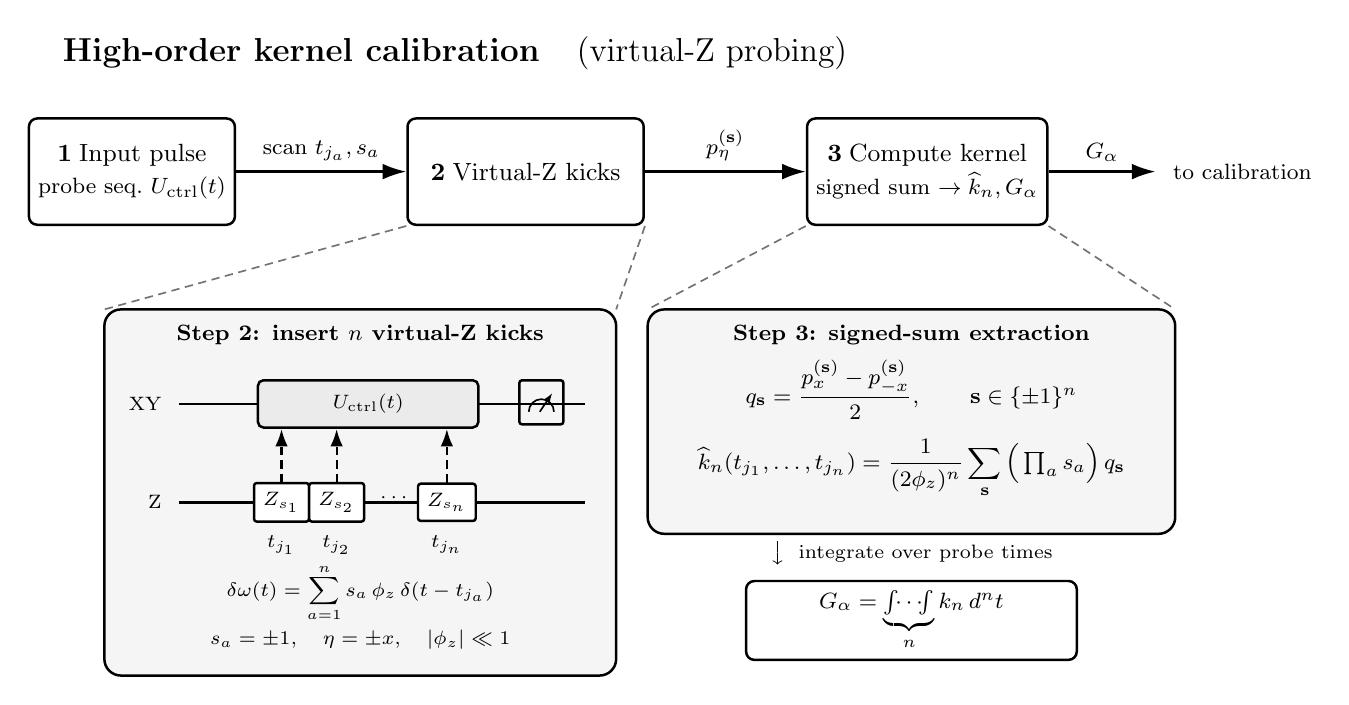
\begin{tikzpicture}[
  x=1cm,
  y=1cm,
  >=Latex,
  font=\large,
  line/.style={draw=black,line width=0.9pt},
  arrow/.style={line,-{Latex[length=3mm,width=2mm]}},
  thinarrow/.style={draw=black,line width=0.55pt,-{Latex[length=2mm,width=1.4mm]}},
  kick/.style={draw=black,line width=0.8pt,densely dashed,-{Latex[length=2.2mm,width=1.6mm]}},
  flowbox/.style={line,rounded corners=3pt,align=center,
                  minimum height=1.35cm,font=\small},
  callout/.style={draw=black!55,line width=0.6pt,densely dashed}
]

% =====================================================================
% Top: brief 3-step flow strip
% =====================================================================
\node[font=\bfseries\large,anchor=west] at (2.55,5.55)
  {High-order kernel calibration\quad\mdseries\large(virtual-Z probing)};

\node[flowbox,minimum width=2.6cm] (s1) at (3.55,4.05)
  {\textbf{1}\;Input pulse\\[0.03cm]{\footnotesize probe seq.\ $U_{\text{ctrl}}(t)$}};
\node[flowbox,minimum width=3.0cm] (s2) at (8.55,4.05)
  {\textbf{2}\;Virtual-Z kicks};
\node[flowbox,minimum width=3.0cm] (s3) at (13.65,4.05)
  {\textbf{3}\;Compute kernel\\[0.03cm]{\footnotesize signed sum $\to\widehat{k}_n,G_\alpha$}};

\draw[arrow] (s1.east) -- node[above,font=\footnotesize] {scan $t_{j_a},s_a$} (s2.west);
\draw[arrow] (s2.east) -- node[above,font=\footnotesize] {$p_\eta^{(\mathbf{s})}$} (s3.west);
\draw[arrow] (s3.east) -- node[above,font=\footnotesize] {$G_\alpha$} (16.55,4.05);
\node[font=\footnotesize,anchor=west] at (16.65,4.05) {to calibration};

% =====================================================================
% Zoom callouts (step 1 stays formal; steps 2 & 3 explode below)
% =====================================================================
\draw[callout] (s2.south west) -- (3.2,2.30);
\draw[callout] (s2.south east) -- (9.7,2.30);
\draw[callout] (s3.south west) -- (10.1,2.30);
\draw[callout] (s3.south east) -- (16.8,2.30);

% =====================================================================
% Panel 2 : virtual-Z kicks (dual-rail: XY abstract + Z explicit)
% =====================================================================
\fill[black!4,rounded corners=6pt] (3.2,-2.35) rectangle (9.7,2.30);
\draw[line,rounded corners=6pt]    (3.2,-2.35) rectangle (9.7,2.30);
\node[anchor=north,font=\footnotesize] at (6.45,2.22)
  {\textbf{Step 2: insert $n$ virtual-Z kicks}};

% --- XY rail: abstract control + meter (no committed waveform) ---
\node[font=\scriptsize,anchor=east] at (4.05,1.10) {XY};
\draw[line] (4.15,1.10) -- (9.30,1.10);
% abstract control block U(t)
\draw[line,fill=black!8,rounded corners=2pt] (5.15,0.80) rectangle (7.95,1.40);
\node[font=\scriptsize] at (6.55,1.10) { $U_{\text{ctrl}}(t)$};
% meter at the end
\begin{scope}[shift={(8.75,1.10)}]
  \draw[line,rounded corners=1pt] (-0.28,-0.26) rectangle (0.28,0.30);
  \draw[line,line width=0.6pt] (-0.16,-0.10) arc (180:0:0.16);
  \draw[line,line width=0.6pt,-{Latex[length=1.3mm,width=0.9mm]}] (-0.02,-0.10) -- (0.14,0.14);
\end{scope}

% --- Z rail: n signed virtual-Z kicks at scanned times ---
\node[font=\scriptsize,anchor=east] at (4.05,-0.15) {Z};
\draw[line] (4.15,-0.15) -- (9.30,-0.15);
\foreach \x/\lab/\tick in {5.45/{Z_{s_1}}/{t_{j_1}}, 6.15/{Z_{s_2}}/{t_{j_2}}, 7.55/{Z_{s_n}}/{t_{j_n}}}{
  \node[line,fill=white,rounded corners=1pt,minimum width=0.52cm,minimum height=0.42cm,
        font=\scriptsize] (\tick) at (\x,-0.15) {$\lab$};
  \node[font=\scriptsize,anchor=north] at (\x,-0.45) {$\tick$};
  % dashed kick: virtual-Z imprints phase on the XY control
  \draw[kick] (\x,0.10) -- (\x,0.78);
}
\node[font=\scriptsize] at (6.90,-0.1) {$\cdots$};

% --- physical content of the kicks ---
\node[font=\scriptsize,anchor=north] at (6.45,-0.80)
  {$\delta\omega(t)=\displaystyle\sum_{a=1}^{n}s_a\,\phi_z\,\delta(t-t_{j_a})$};
\node[font=\scriptsize,anchor=north] at (6.45,-1.65)
  {$s_a=\pm1,\quad \eta=\pm x,\quad |\phi_z|\ll1$};

% =====================================================================
% Panel 3 : compute kernel (signed sum -> k_n -> G_alpha), no heatmap
% =====================================================================
\fill[black!4,rounded corners=6pt] (10.1,-0.55) rectangle (16.8,2.30);
\draw[line,rounded corners=6pt]    (10.1,-0.55) rectangle (16.8,2.30);
\node[anchor=north,align=center,font=\footnotesize] at (13.45,2.22)
  {\textbf{Step 3: signed-sum extraction}\vspace{0.4cm}\\[0.16cm]
   $q_{\mathbf{s}}=\dfrac{p_x^{(\mathbf{s})}-p_{-x}^{(\mathbf{s})}}{2},\qquad
    \mathbf{s}\in\{\pm1\}^{n}$\\[0.22cm]
   $\widehat{k}_n(t_{j_1},\dots,t_{j_n})=
     \dfrac{1}{(2\phi_z)^{n}}\displaystyle\sum_{\mathbf{s}}
     \Big(\textstyle\prod_a s_a\Big)\,q_{\mathbf{s}}$\\[0.20cm]};
  % {\footnotesize e.g.\ $\widehat{k}_2=\dfrac{q_{++}-q_{+-}-q_{-+}+q_{--}}{(2\phi_z)^2}$}};

% integrate -> G_alpha
\node[font=\scriptsize] at (13.45,-0.80) {$\big\downarrow$\;\ integrate over probe times};
\node[line,rounded corners=3pt,align=center,font=\footnotesize,
      minimum width=4.2cm,minimum height=0.85cm] (gbox) at (13.45,-1.65)
  {$G_\alpha=\underbrace{\textstyle\int\!\!\cdots\!\!\int}_{n} k_n\,d^{n}t$};

% =====================================================================
% cost footnote
% =====================================================================
% \node[font=\footnotesize,anchor=north west] at (3.20,-2.55)
%   {Cost: $2^{n}M^{n}N_{\mathrm{shot}}$ settings ($n$-D scan over probe times $\times$ sign patterns).};

\end{tikzpicture}
\end{document}
